\documentclass{beamer}
\usepackage[italian]{babel}
\usepackage{xcolor}

\DeclareMathOperator{\lcm}{lcm}

\title{Presentazione PHPC}
\author{Pierluigi Supino \and Rodolfo Diana \and Salvatore Di Gennaro}

\usetheme{default}
\begin{document}
\begin{frame}
    \titlepage
\end{frame}

\begin{frame}{Implementazione}{SUMMA}
    \begin{itemize}
        \item Scalable Universal Matrix Multiplication Algorithm (SUMMA)
        \item Algoritmo efficiente e scalabile per ogni numero di processi
        \item Si dispongono i processi in una griglia $r \times c$
    \end{itemize}
    \begin{figure}
        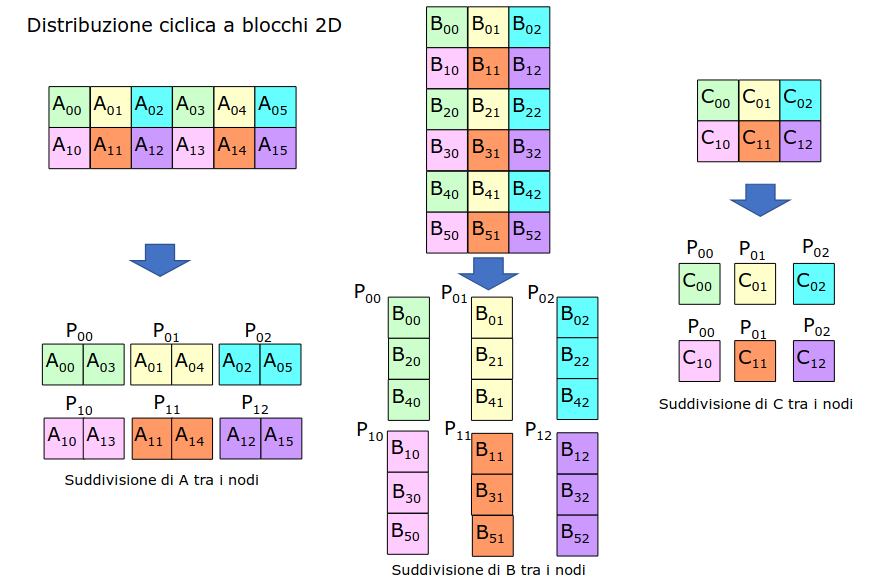
\includegraphics[width=0.5\linewidth]{imgs/summa.png}
        \caption{Distribuzione SUMMA}
    \end{figure}
\end{frame}

\begin{frame}{Implementazione}{SUMMA}
    Semplificazioni e assunzioni effettuate:
    \begin{itemize}
        \item solo matrici quadrate $n \times n$
        \item lato delle matrici perfettamente divisibile per $\lcm(r,c)$
        \item matrici come array contigui \textit{row-major}
        \item matrici di input di ogni processo contengono già i dati necessari
    \end{itemize}
\end{frame}

\begin{frame}{Implementazione}{Multi-GPU}
    \begin{itemize}
        \item Più GPU per processo: come suddividere il lavoro?
              \begin{itemize}
                  \item Vogliamo eseguire le operazioni in parallelo
                        \begin{itemize}
                            \item Evitare conflitti di memoria da serializzare
                            \item Nessuna funzione bloccante
                        \end{itemize}
              \end{itemize}
        \item Possibili soluzioni:
              \begin{itemize}
                  \item Pattern fork-join con ogni thread che gestisce una GPU
                  \item \color{red} Utilizzo dei metodi async e degli stream di CUDA
              \end{itemize}
    \end{itemize}
\end{frame}


\begin{frame}{Implementazione}{Multi-GPU - CUDA}
    \begin{itemize}
        \item CUDA stream: code di operazioni da gestire in sequenza
              \begin{itemize}
                  \item Operazioni in stream diversi potrebbero essere eseguite in concorrenza
                  \item Operazioni in stream diversi potrebbero essere alternate
                  \item Se non viene specificato uno stream viene usato lo stream 0 (bloccante)
              \end{itemize}
        \item I trasferimenti sono davvero asincroni solo se la memoria indirizzata è \textit{page-locked}
              \begin{itemize}
                  \item cudaMallocHost
                  \item cudaHostRegister/cudaHostUnregister
              \end{itemize}
    \end{itemize}
\end{frame}

\begin{frame}{Implementazione}{cuBLAS}
    \begin{itemize}
        \item BLAS: specifiche di routine di basso livello per operazioni algebriche (vettori, matrici)
        \item cuBLAS: implementazione ottimizzata per GPU NVIDIA
              \begin{itemize}
                  \item Per compatibilità con Fortran si aspetta ordine column-major
                  \item $\mathbf{C}^T=(\mathbf{B}\mathbf{A})^T$
              \end{itemize}
        \item \color{red} cuBLASXt: estensione per supportare ambienti multi-GPU
    \end{itemize}
\end{frame}


\end{document}